\documentclass{beamer}

\usetheme{metropolis}

\usepackage{appendixnumberbeamer}
\usepackage{makecell}
\usepackage{graphicx}
\usepackage{makecell}
\usepackage{amsmath}
\usepackage{hyperref}
\usepackage{booktabs}
\usepackage{blkarray} % random math 
\usepackage[mathrm=sym]{unicode-math}
\setmathfont{Fira Math}
\setmathfont{Latin Modern Math}[range={\vdots, \ddots, \top}]

% --- Bibliography ---
\usepackage[authordate, backend=biber, ibidtracker=false]{biblatex-chicago} % packages
\bibliography{key_bridge} % .bib file
\setbeamertemplate{bibliography item}{}

\def\sym#1{\ifmmode^{#1}\else\(^{#1}\)\fi}
\numberwithin{figure}{section} % number figure with section number
\numberwithin{table}{section} % number table with section number

\title{Vulnerability of Urban Road Systems}
\subtitle{A Network Analysis of the Baltimore Bridge Collapse}
\author{Gavin Engelstad}
\date{Spring 2024}
\institute{Macalester College}

\begin{document}

\maketitle

\section{Background}

\begin{frame}{The Event}
    \begin{figure}
        \centering
        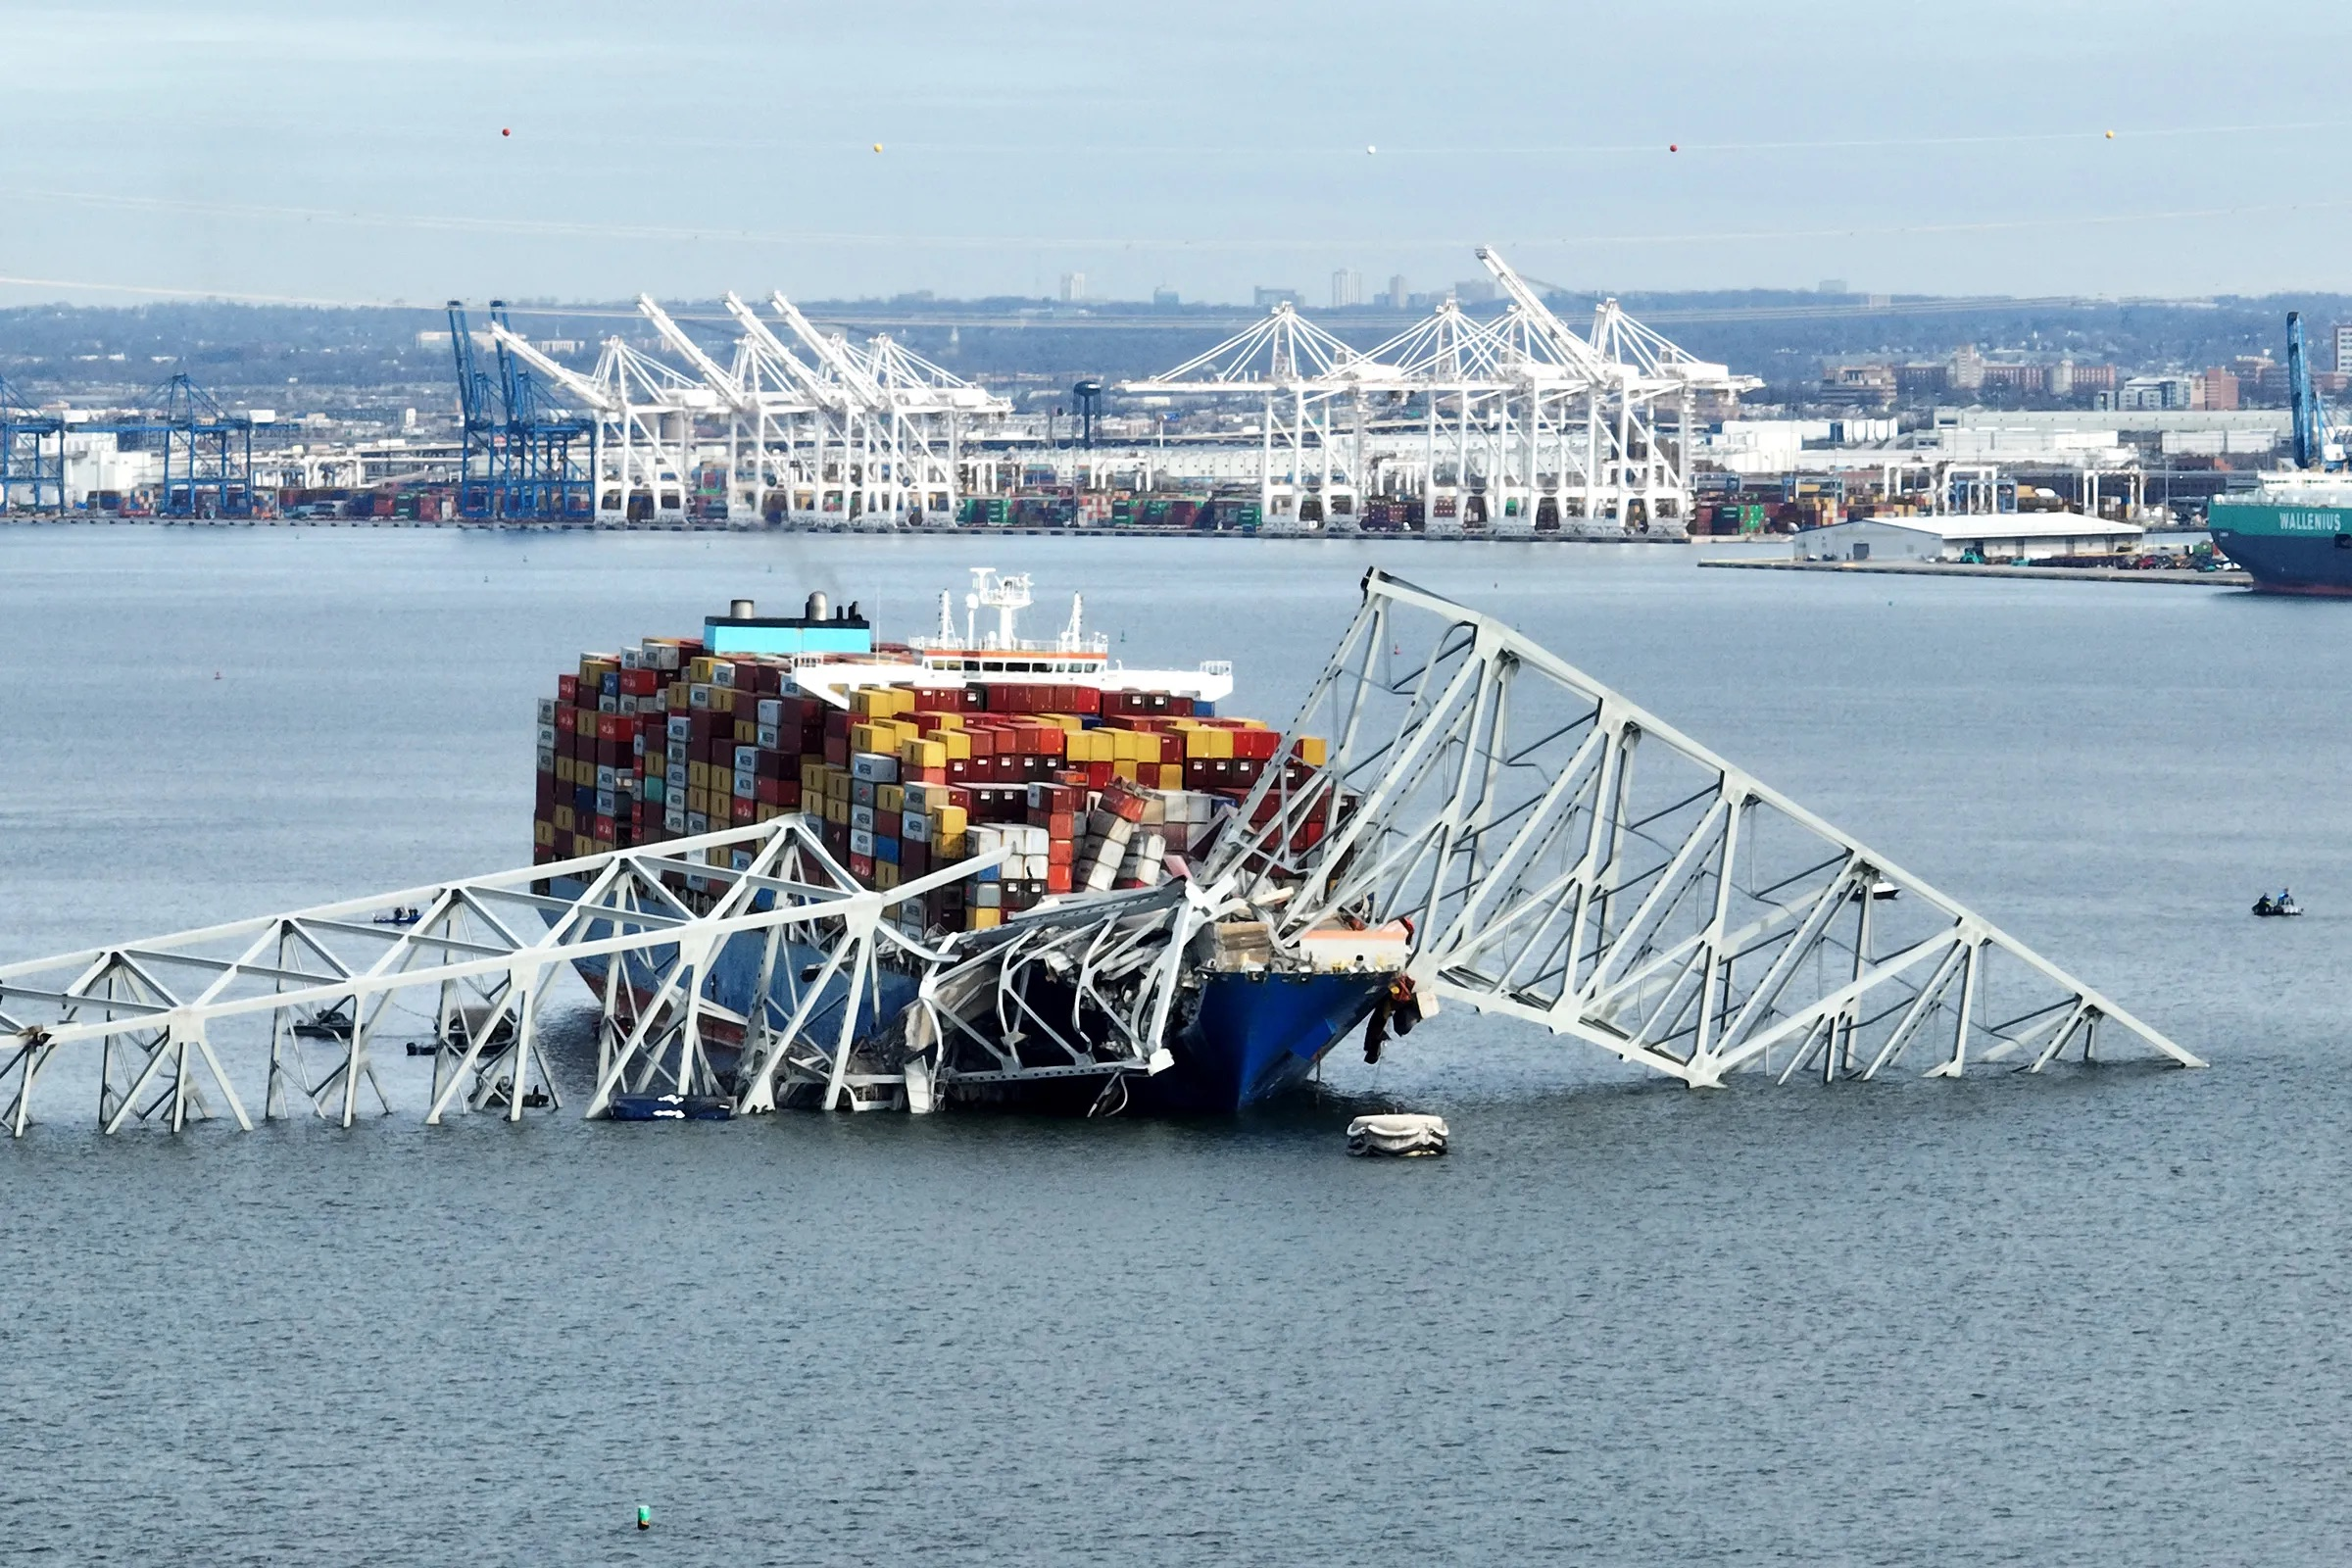
\includegraphics[width=0.9\textwidth]{pics/Balitmore-Bridge-Collapse.jpeg} \\
        {\scriptsize On March 26, 2024, the \textit{Dali} struck and collapsed the Francis Scott Key Bridge}
    \end{figure}
\end{frame}

\begin{frame}{Key Bridge}
    \begin{columns}
        \begin{column}{0.5\textwidth}
            The Francis Scott Key Bridge is part of I-695, or Baltimore Beltway

            It's an important part of the Balitmore Road System
            \begin{itemize}
                \item 30,000 cars travel across it every day
                \item Spans the entire port of Baltimore (1.6 Miles)
            \end{itemize}
        \end{column}

        \begin{column}{0.5\textwidth}
            \begin{figure}
                \centering
                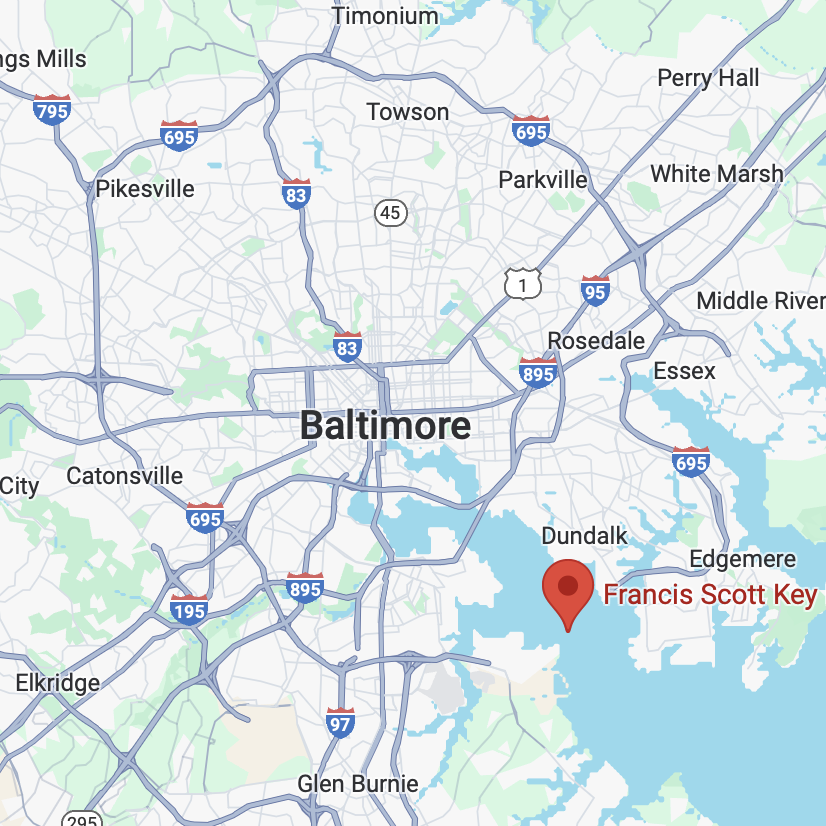
\includegraphics[width=\textwidth]{pics/map_of_bridge.png} \\
                {\tiny Screenshot from Google Maps}
            \end{figure}
        \end{column}
    \end{columns}
\end{frame}

\begin{frame}{Questions}
    \begin{center}
        How did the bridge collapse affect the road network as whole?

        Where are these effects concentrated?
    \end{center}
\end{frame}


\section{Empirical Strategy}

\subsection{The Network}

\begin{frame}{The Network (1/3)}
    Create a network using intersections as nodes and road segments as edges

    The ``Primal Approach'' {\tiny \parencite{Porta06}}

    Compare this network with and without the bridge edges
\end{frame}

\begin{frame}{The Network (2/3)}
    We get our network from OSMnx, a Python library that uses Open Street Maps to create a directed multigraph for any road system in the world {\tiny \parencite{Boeing17}}

    7 counties in the BMA: Anne Arundel, Baltimore City, Baltimore County, Carroll, Harford, Howard, and Queen Anne's County

    Filter out 272 nodes that aren't a part of the largest strongly connected component

    End up with a network with
    \begin{itemize}
        \item 91,300 nodes (intersections)
        \item 218,842 edges (road segments)
        \item 4 collapsed road segments
    \end{itemize}
\end{frame}

\begin{frame}{The Network (3/3)}
    \begin{columns}
        \begin{column}{0.5\textwidth}
            \begin{figure}
                \centering
                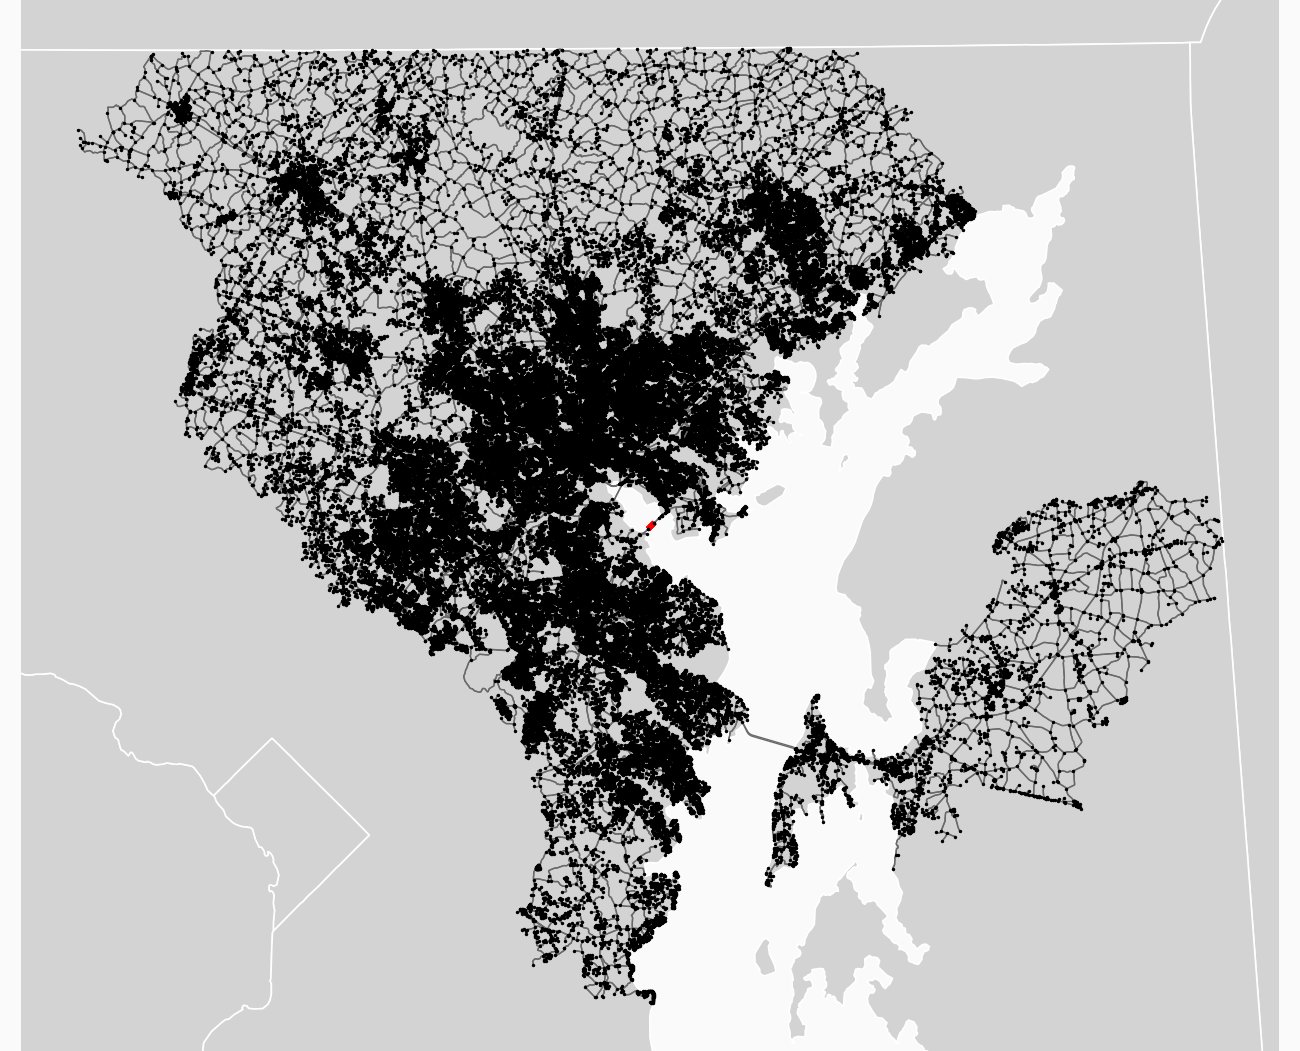
\includegraphics[width=\textwidth]{maps/full_network.png} \\
                {\scriptsize Total BMA Network}
            \end{figure}
        \end{column}

        \begin{column}{0.5\textwidth}
            \begin{figure}
                \centering
                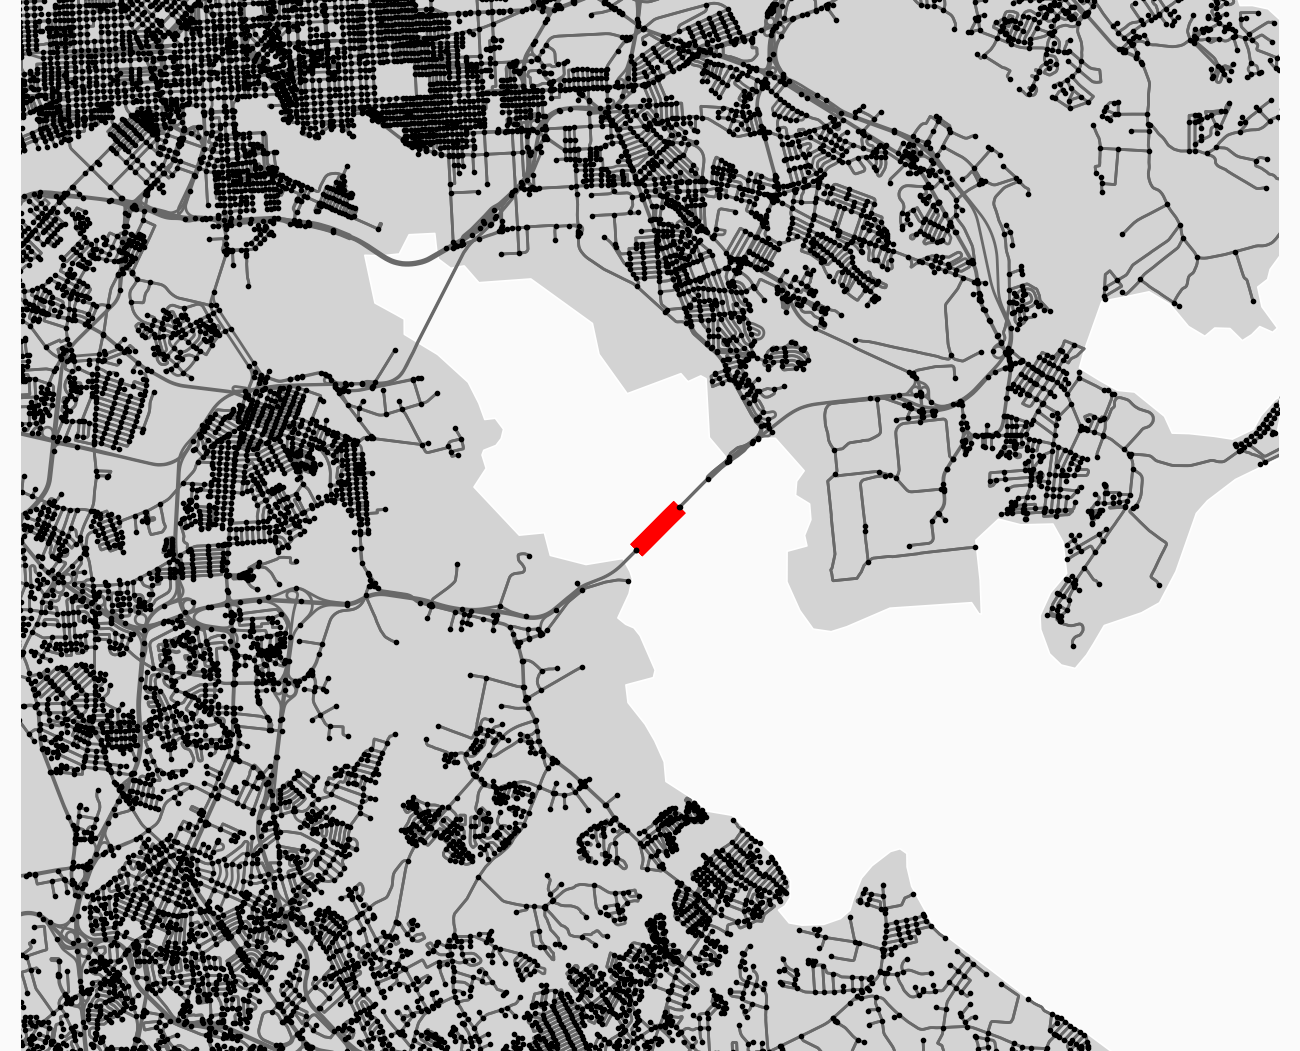
\includegraphics[width=\textwidth]{maps/zoomed_network.png} \\
                {\scriptsize Zoomed In to Key Bridge}
            \end{figure}
        \end{column}
    \end{columns}

    \begin{center}
    {\footnotesize Key Bridge highlighted in red.}
    \end{center}
\end{frame}

\subsection{Methods}

\begin{frame}{Method}
    Analyze global network effects using average shortest path length {\tiny \parencites{Xeumei10}{Kaub24}}

    Analyze local effects using Multiple Centrality Analysis (MCA) {\tiny \parencites{Porta06}{Porta07}{Barthelemy09}{Jayaweera17}}
    \begin{itemize}
        \item Eigenvector Centrality: High traffic ``important'' areas
        \item Betweenness Centrality: Important routes
        \item Closeness Centrality: Areas with high land use, can have issues on a bounded network
        \item Straightness Centrality: Important routes and land use
    \end{itemize}

   Analyze the impacted paths for even more localized effects
\end{frame}

\begin{frame}{Straightness Centrality}
    Straightness Centrality is a measure specific to spatial networks that measures how directly you can travel to other nodes

    \begin{equation*}
        C_i^S = \frac{1}{n-1} \sum_{j \in N, j \neq i} \frac{d_{i, j}^\text{Eucl}}{d_{i, j}}
    \end{equation*}
\end{frame}


\section{Results}

\begin{frame}{Average Shortest Path}
    The average shortest path was only marginally affected
    
    \begin{table}
        \centering
        \begin{tabular}{ccccc}
            \toprule
            \textbf{Before Collapse} & \textbf{After Collapse} & \textbf{Difference} & \textbf{\% Difference} \\
            \midrule
            26.3 & 26.4 & 0.09 & 0.003 \\
            \bottomrule
        \end{tabular}
        {\scriptsize Length of the average shortest path in the BMA road network (Miles)}
    \end{table}
\end{frame}

\begin{frame}{MCA: Eigenvector Centrality}
    \begin{columns}
        \begin{column}{0.33\textwidth}
            \begin{figure}
                \centering
                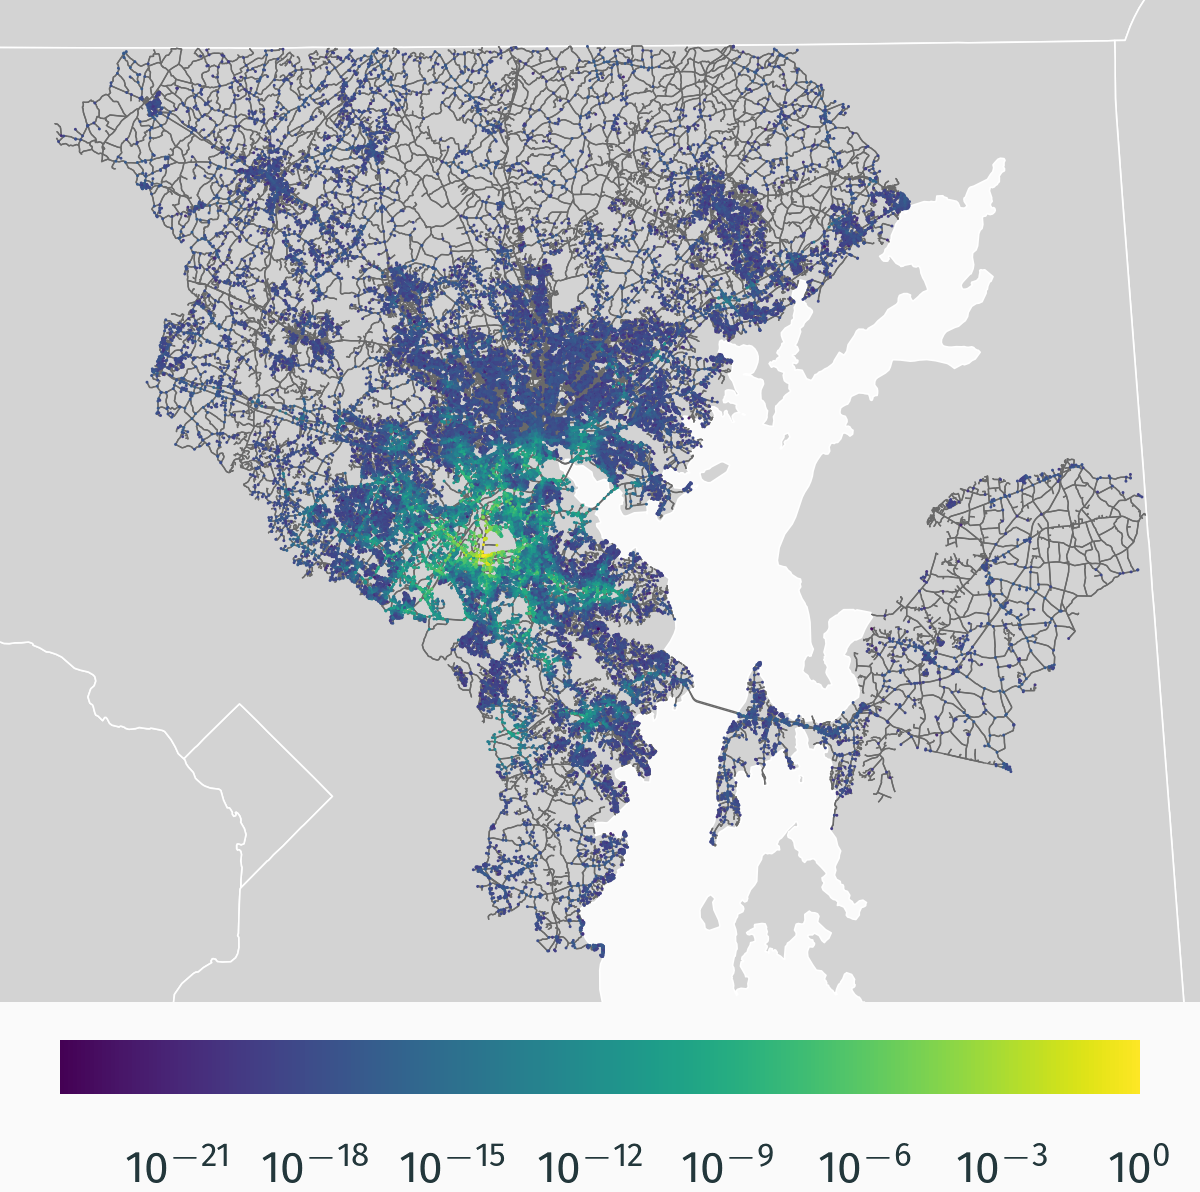
\includegraphics[width=\textwidth]{maps/eigenvector_w_bridge.png}
                {\scriptsize Eigenvector Centrality before the collapse}
            \end{figure}
        \end{column}

        \begin{column}{0.33\textwidth}
            \begin{figure}
                \centering
                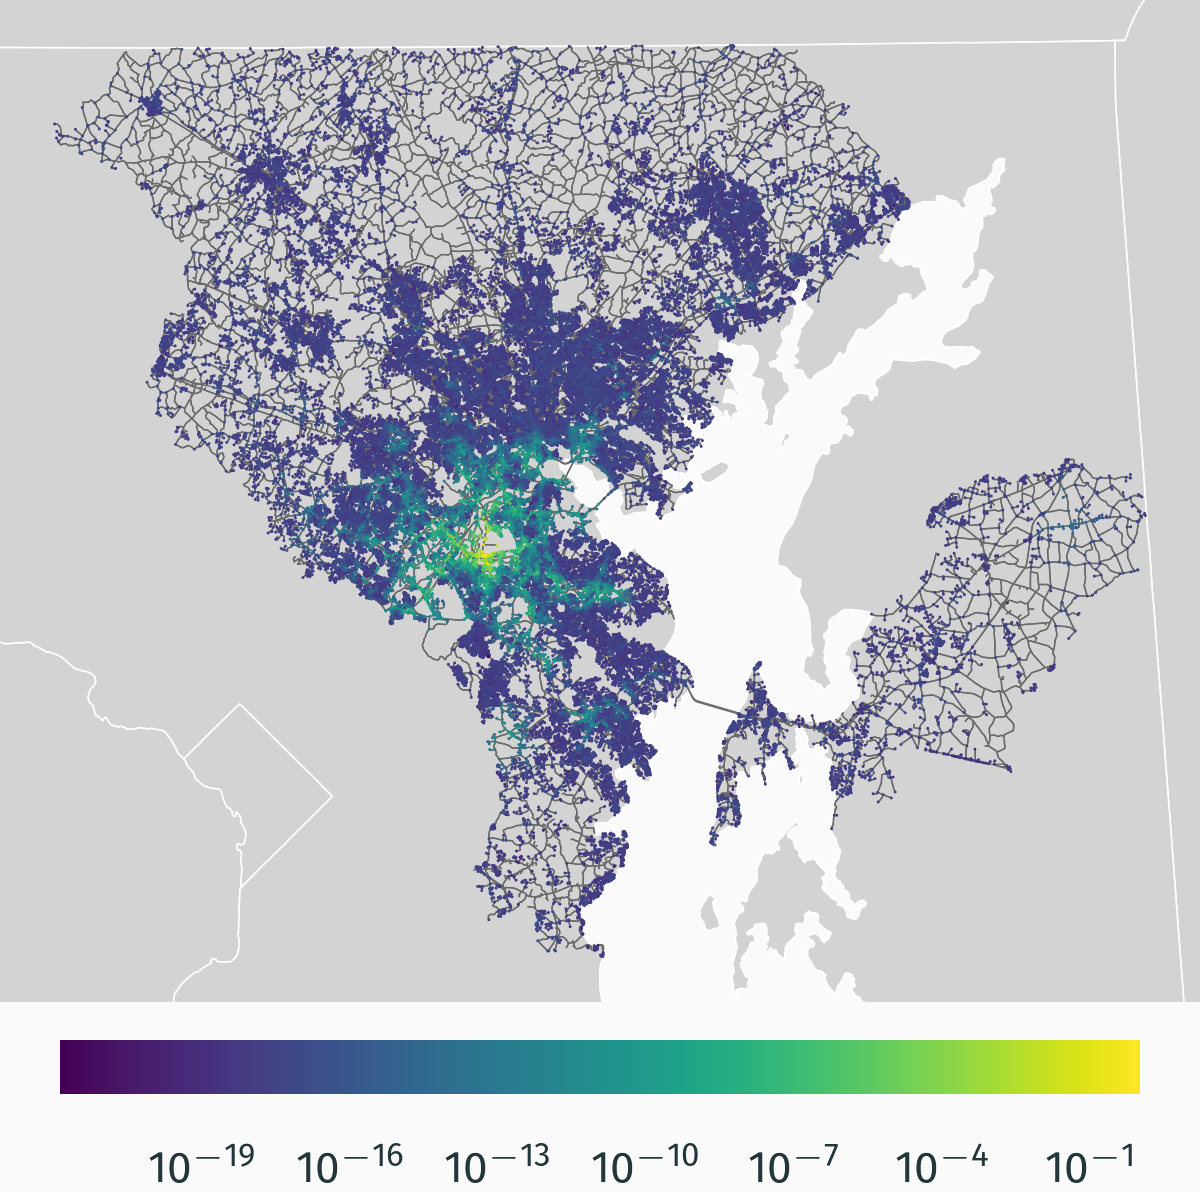
\includegraphics[width=\textwidth]{maps/eigenvector_wo_bridge.png}
                {\scriptsize Eigenvector Centrality after the collapse}
            \end{figure}
        \end{column}

        \begin{column}{0.33\textwidth}
            \begin{figure}
                \centering
                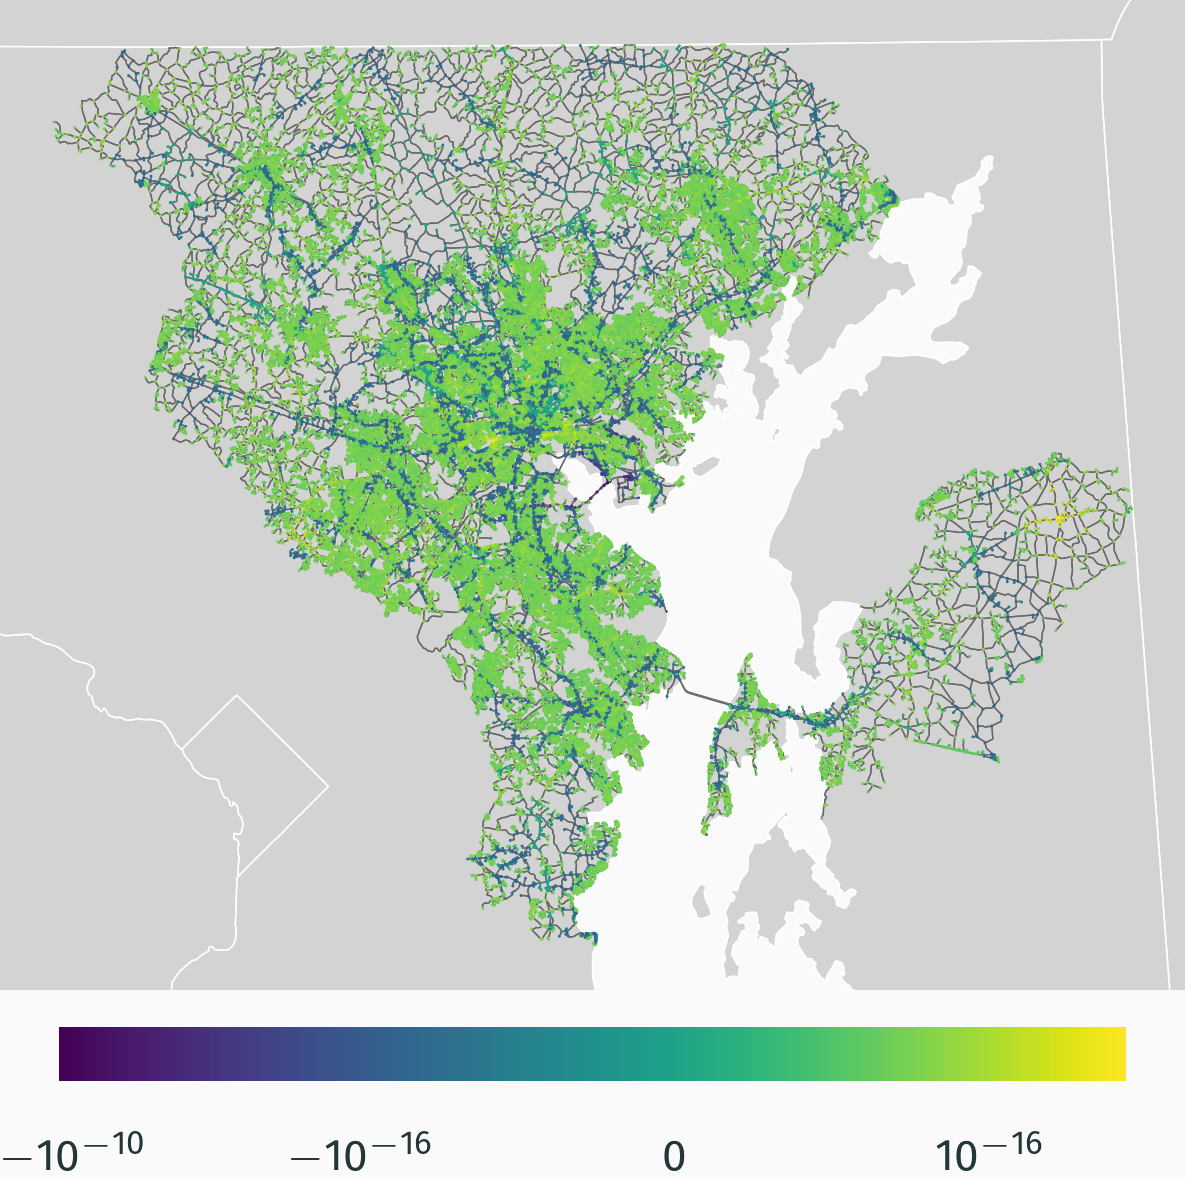
\includegraphics[width=\textwidth]{maps/eigenvector_diff.png}
                {\scriptsize Change in Eigenvector Centrality}
            \end{figure}
        \end{column}
    \end{columns}
\end{frame}

\begin{frame}{MCA: Betweenness Centrality}
    \begin{columns}
        \begin{column}{0.33\textwidth}
            \begin{figure}
                \centering
                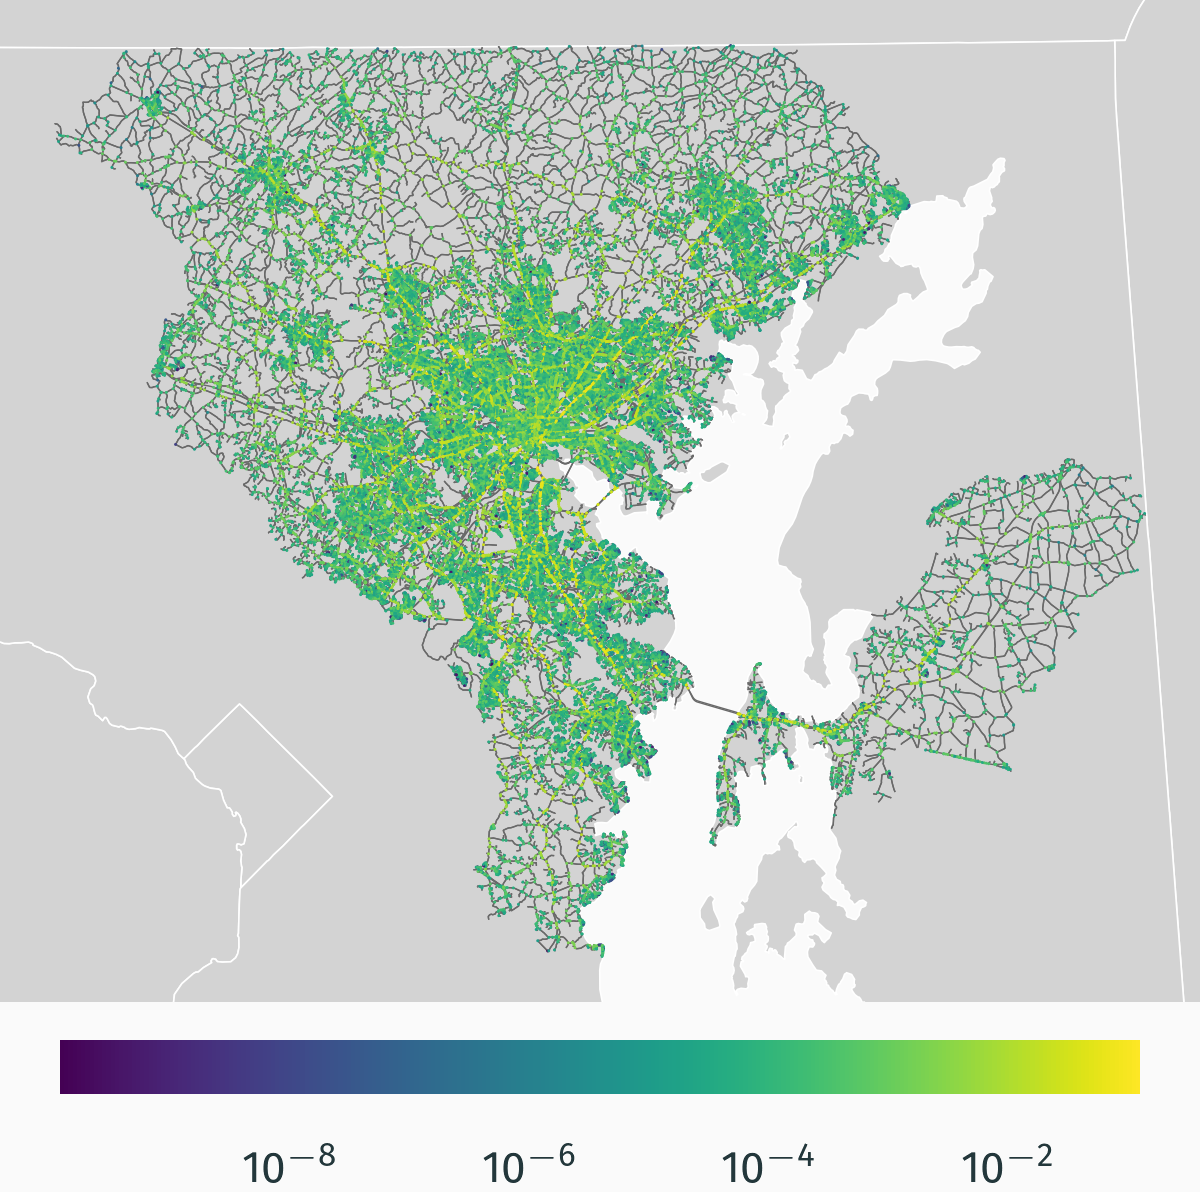
\includegraphics[width=\textwidth]{maps/betweenness_w_bridge.png}
                {\scriptsize Betweenness Centrality before the collapse}
            \end{figure}
        \end{column}

        \begin{column}{0.33\textwidth}
            \begin{figure}
                \centering
                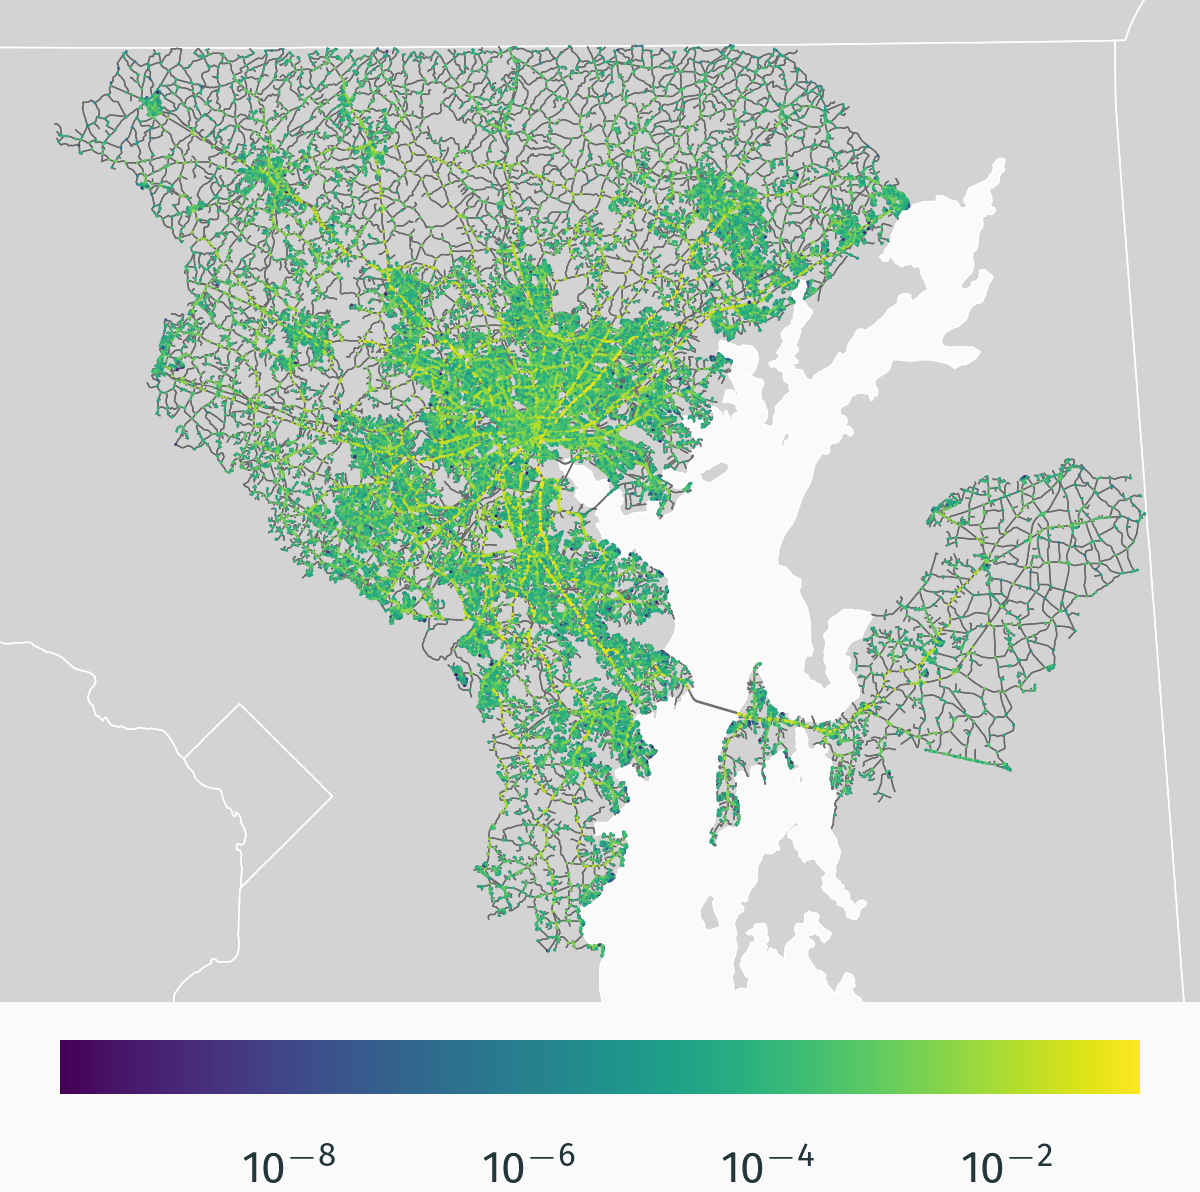
\includegraphics[width=\textwidth]{maps/betweenness_wo_bridge.png}
                {\scriptsize Betweenness Centrality after the collapse}
            \end{figure}
        \end{column}

        \begin{column}{0.33\textwidth}
            \begin{figure}
                \centering
                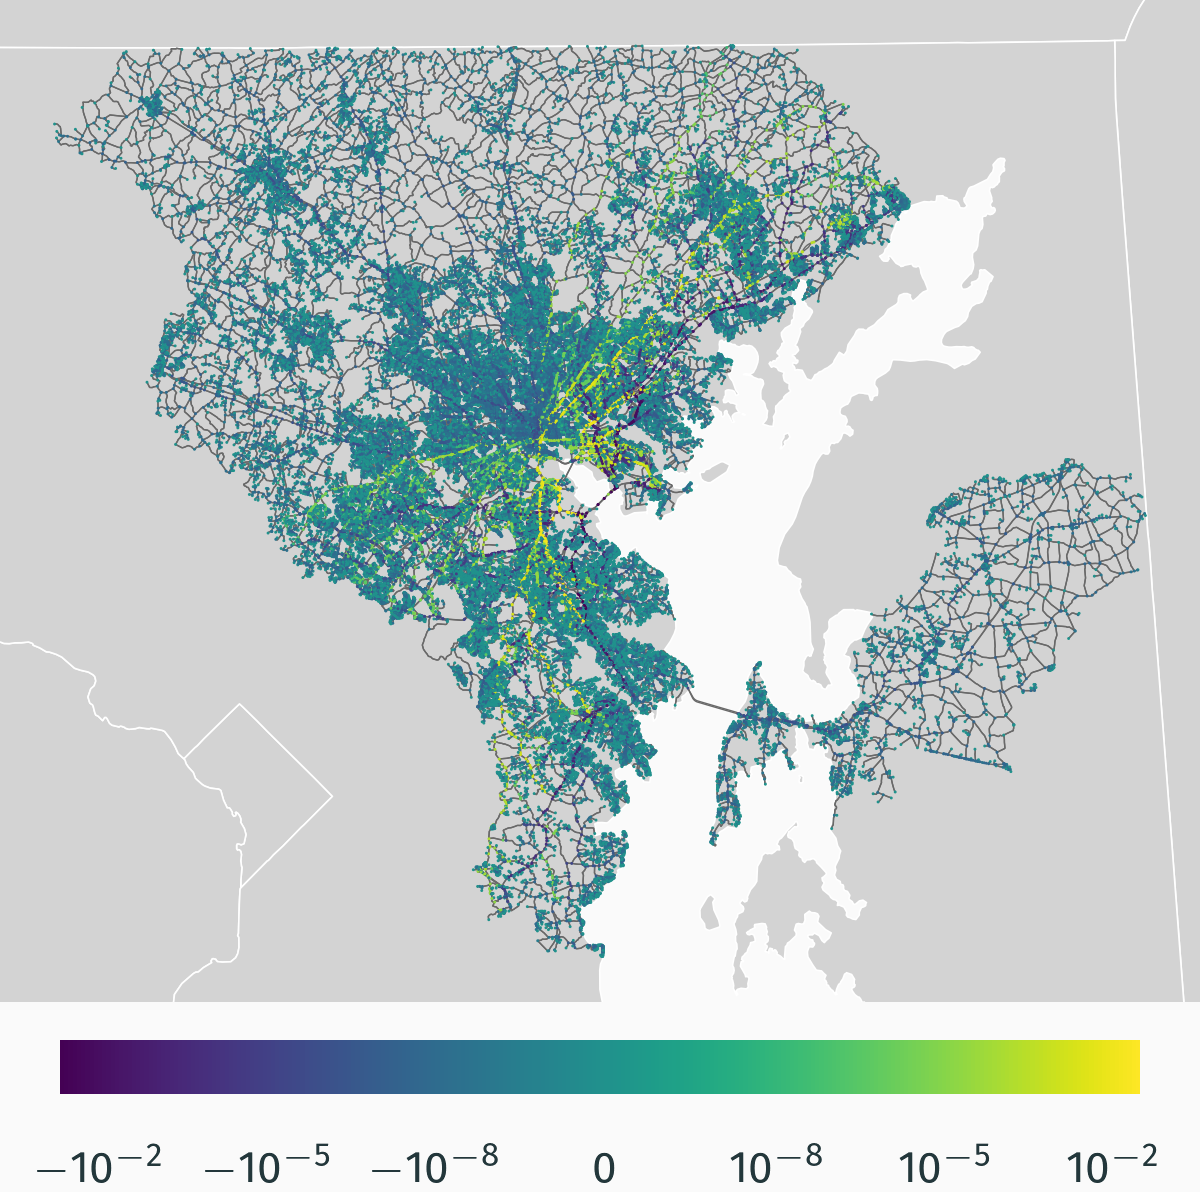
\includegraphics[width=\textwidth]{maps/betweenness_diff.png}
                {\scriptsize Change in Betweenness Centrality}
            \end{figure}
        \end{column}
    \end{columns}
\end{frame}

\begin{frame}{MCA: Closeness Centrality}
    \begin{columns}
        \begin{column}{0.33\textwidth}
            \begin{figure}
                \centering
                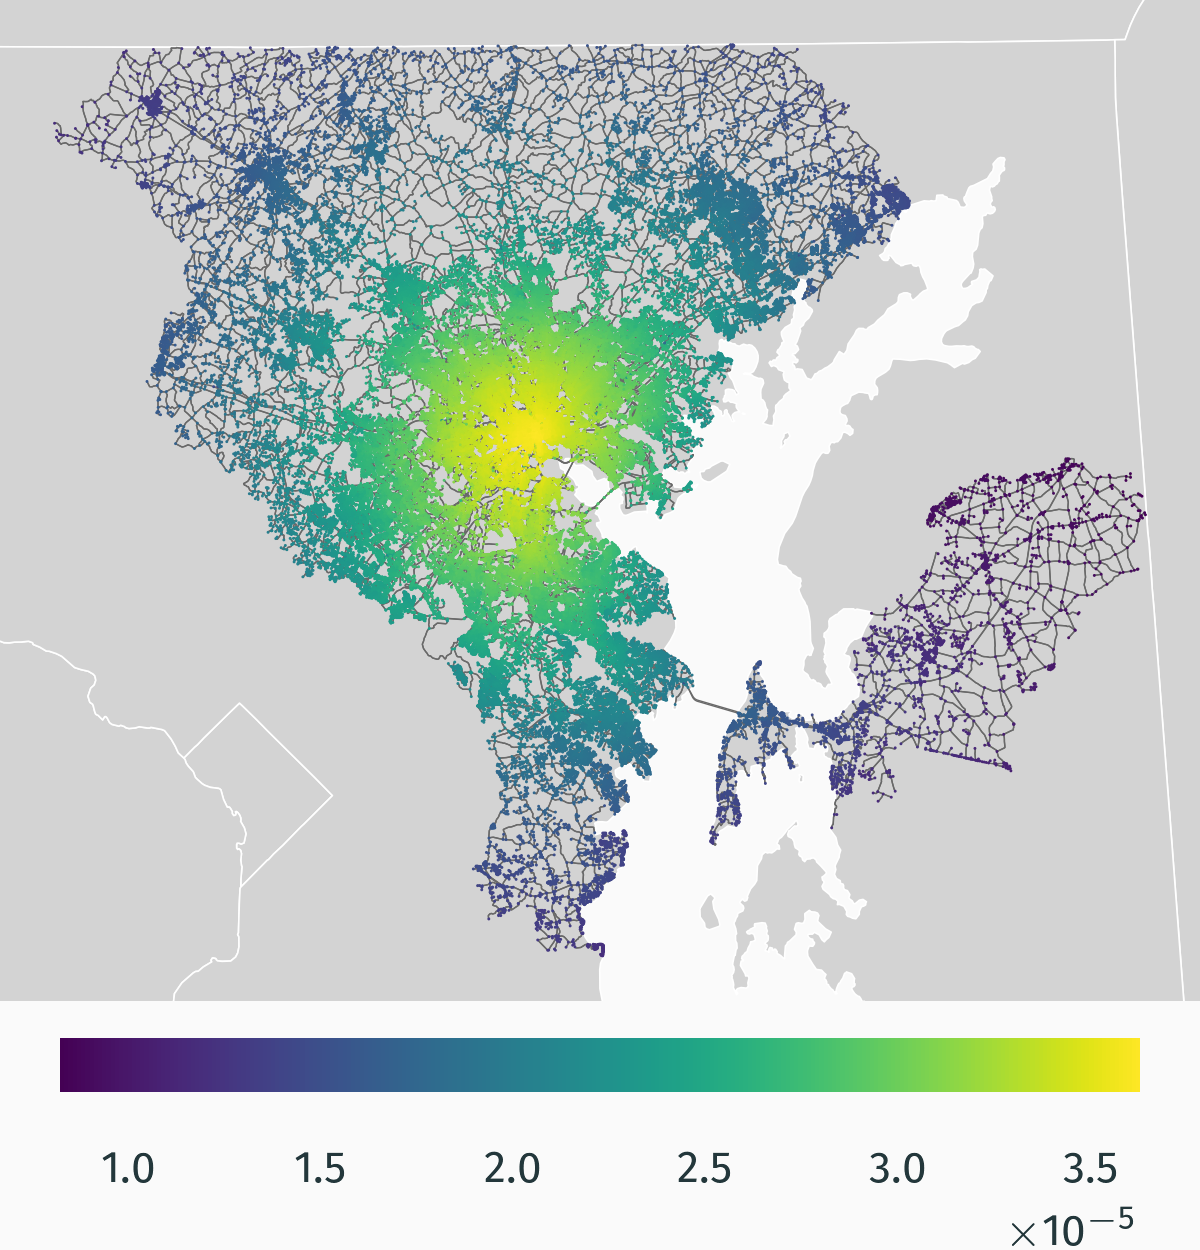
\includegraphics[width=\textwidth]{maps/closeness_w_bridge.png}
                {\scriptsize Closeness Centrality before the collapse}
            \end{figure}
        \end{column}

        \begin{column}{0.33\textwidth}
            \begin{figure}
                \centering
                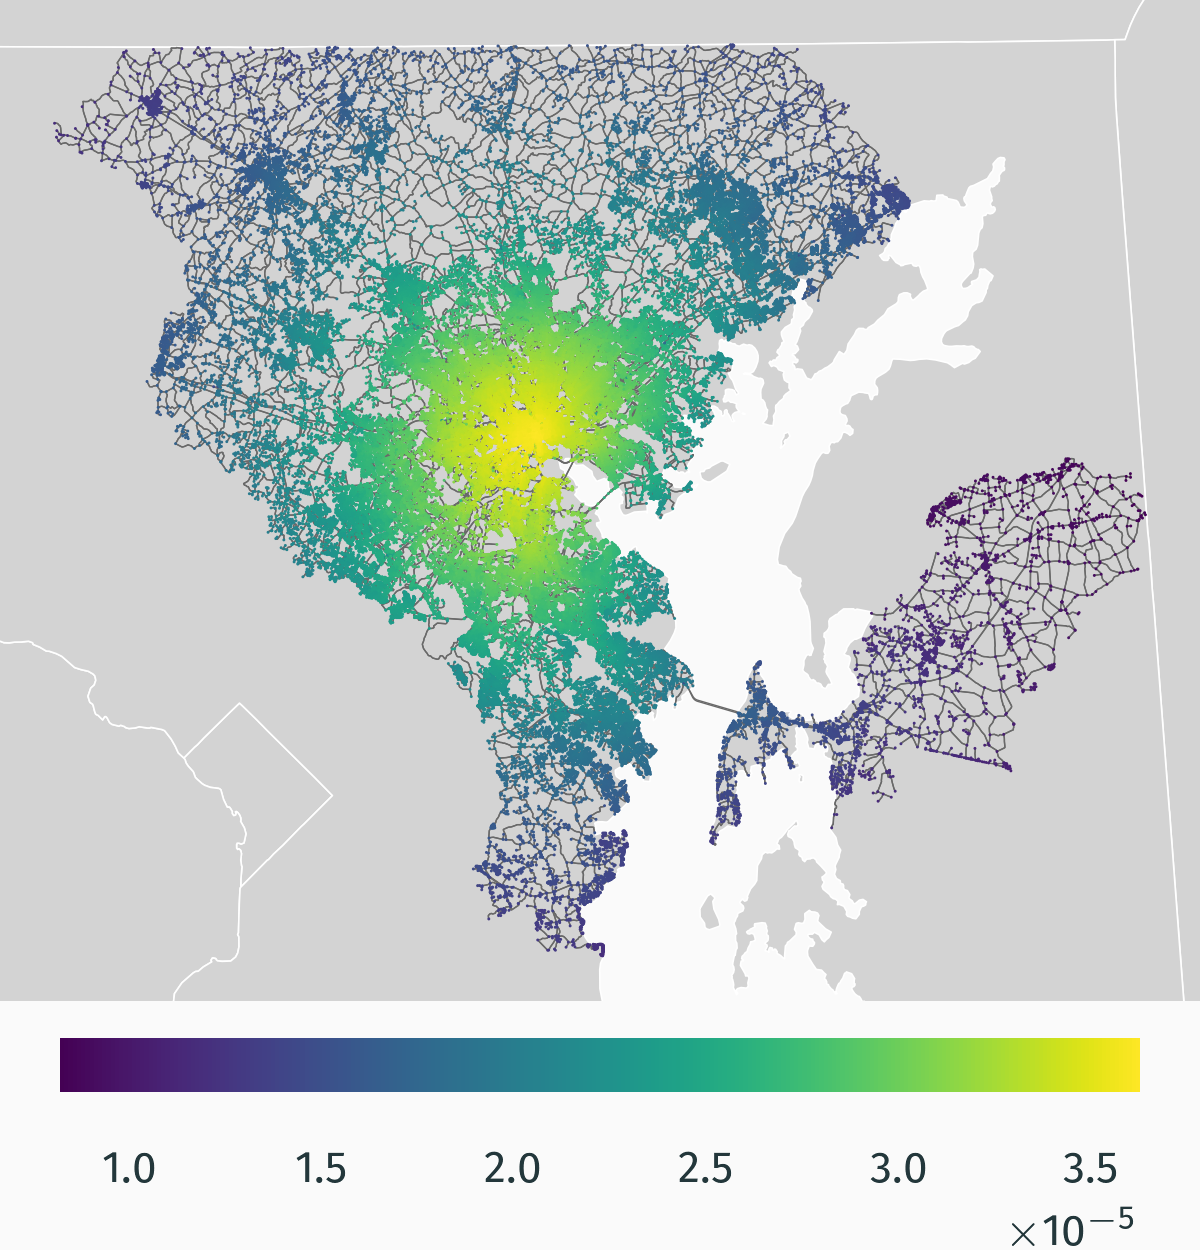
\includegraphics[width=\textwidth]{maps/closeness_wo_bridge.png}
                {\scriptsize Closeness Centrality after the collapse}
            \end{figure}
        \end{column}

        \begin{column}{0.33\textwidth}
            \begin{figure}
                \centering
                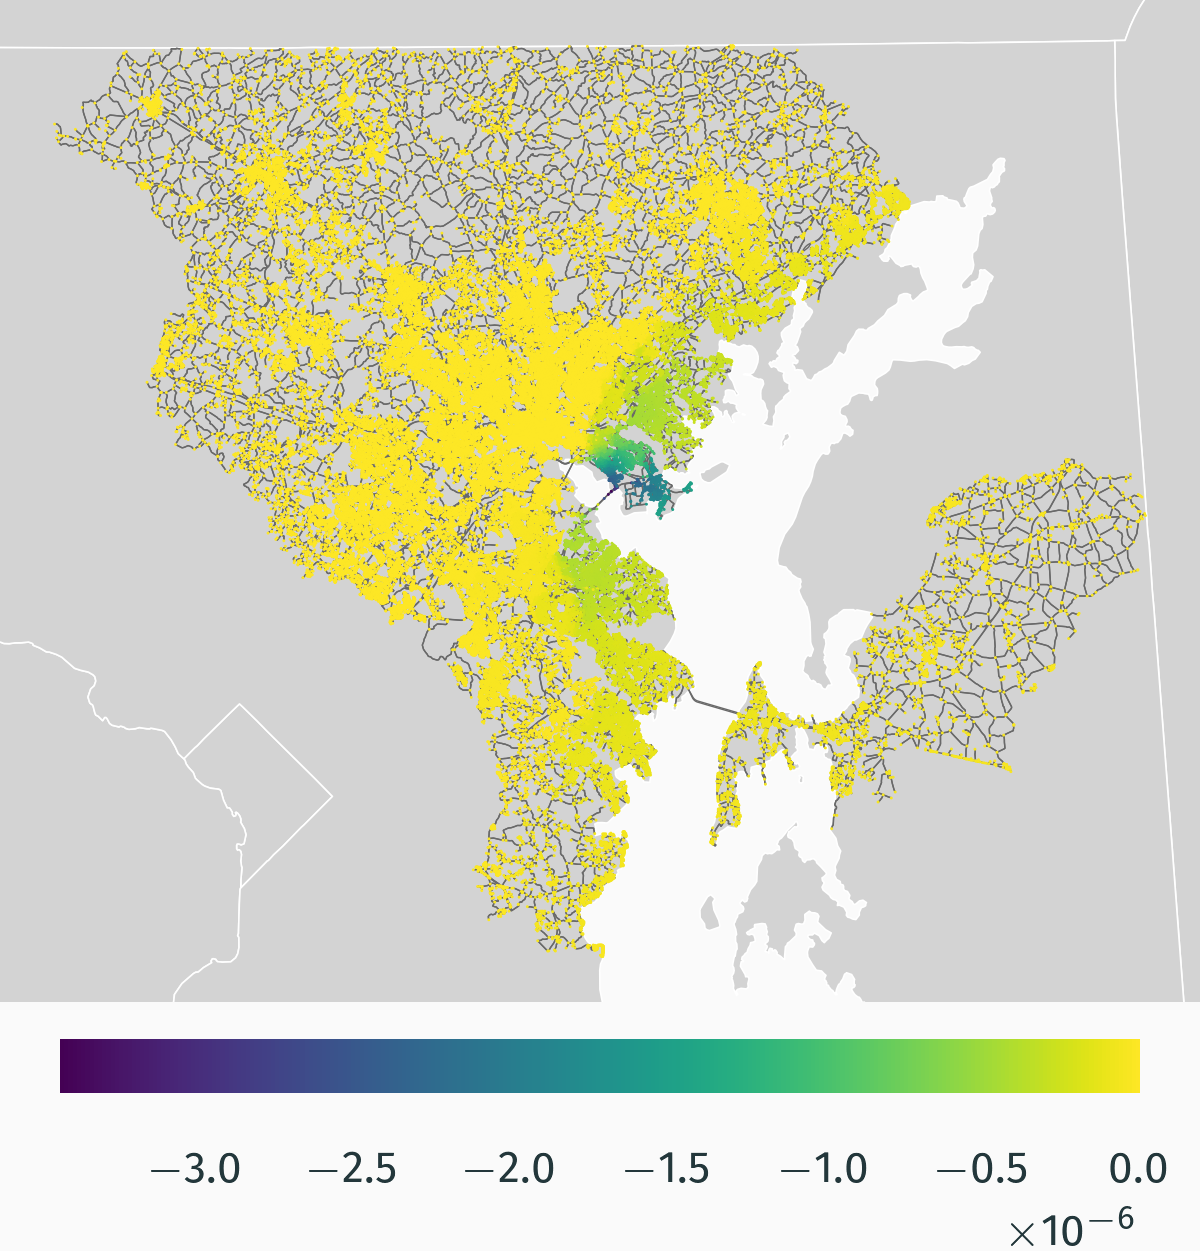
\includegraphics[width=\textwidth]{maps/closeness_diff.png}
                {\scriptsize Change in Closeness Centrality}
            \end{figure}
        \end{column}
    \end{columns}
\end{frame}

\begin{frame}{MCA: Straightness Centrality}
    \begin{columns}
        \begin{column}{0.33\textwidth}
            \begin{figure}
                \centering
                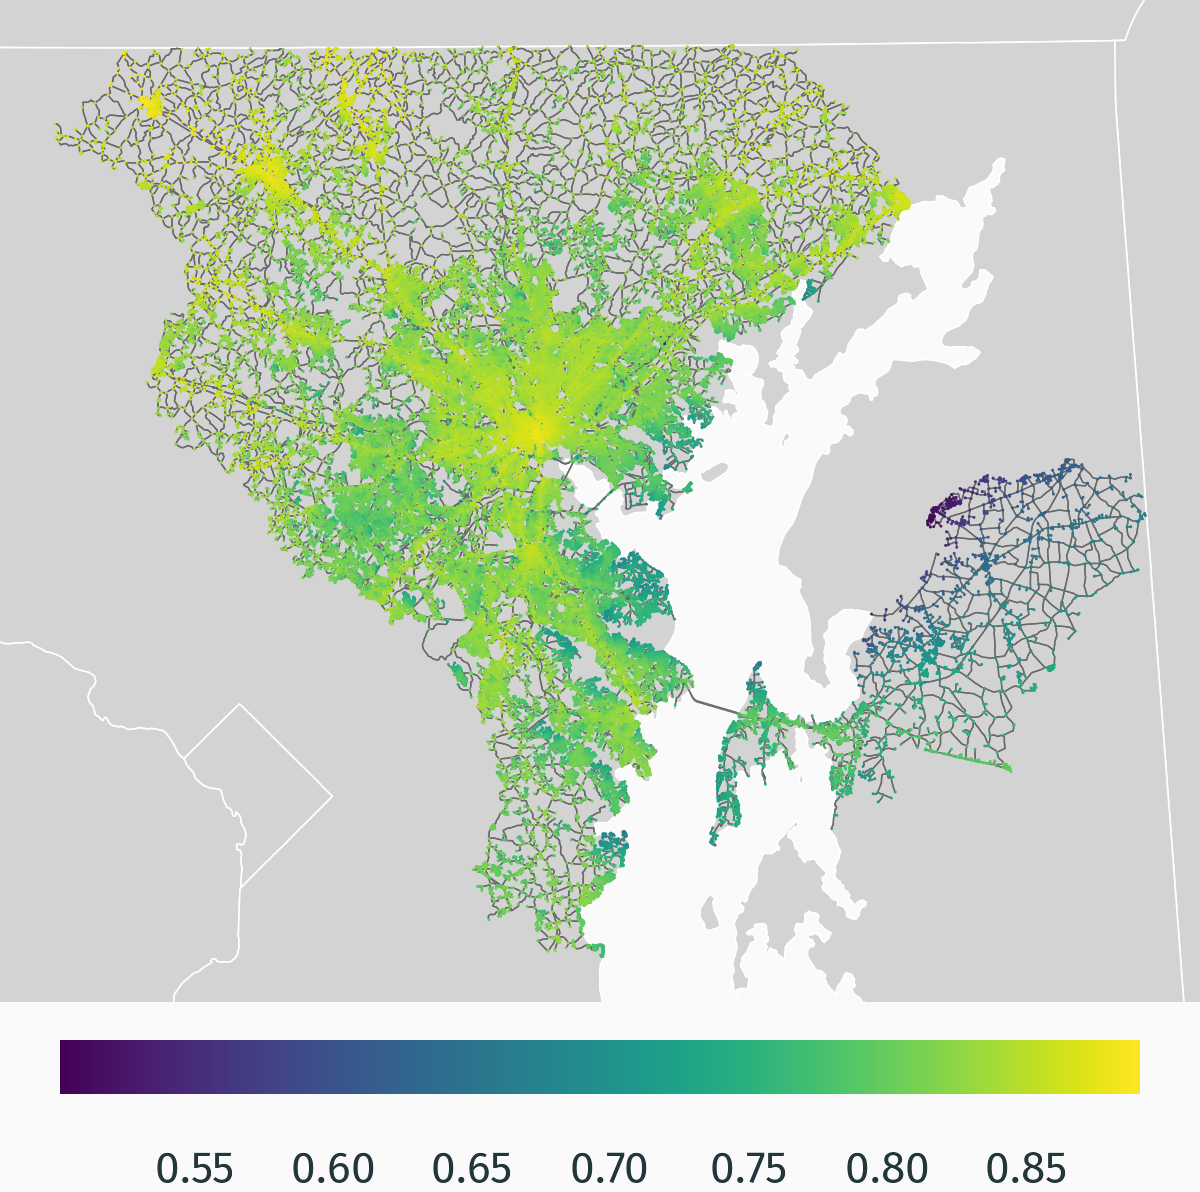
\includegraphics[width=\textwidth]{maps/straightness_w_bridge.png}
                {\scriptsize Straightness Centrality before the collapse}
            \end{figure}
        \end{column}

        \begin{column}{0.33\textwidth}
            \begin{figure}
                \centering
                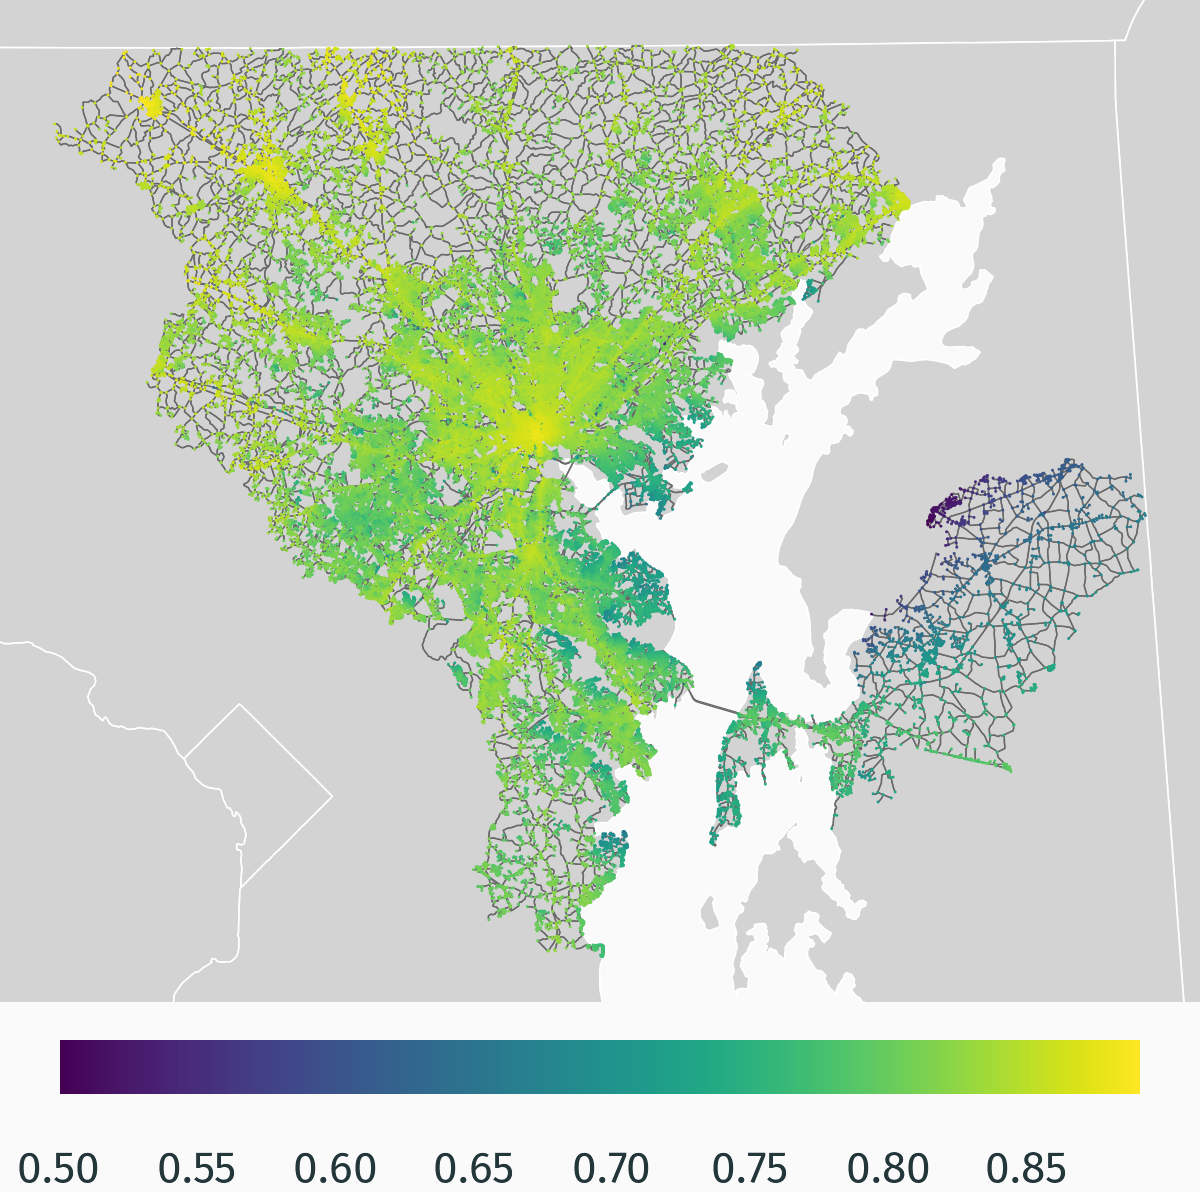
\includegraphics[width=\textwidth]{maps/straightness_wo_bridge.png}
                {\scriptsize Straightness Centrality after the collapse}
            \end{figure}
        \end{column}

        \begin{column}{0.33\textwidth}
            \begin{figure}
                \centering
                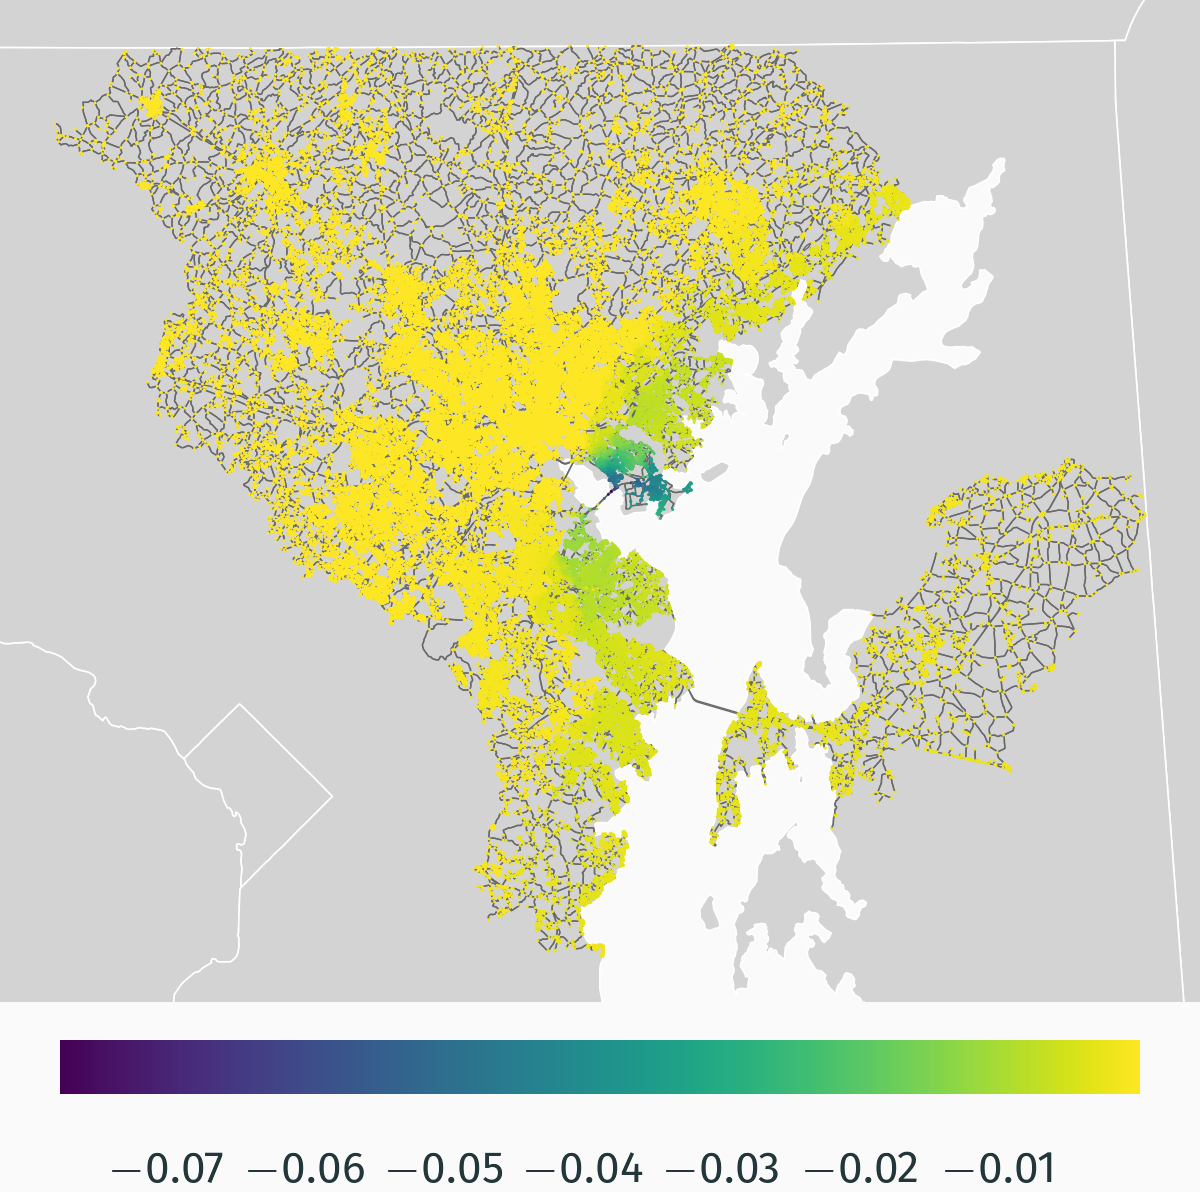
\includegraphics[width=\textwidth]{maps/straightness_diff.png}
                {\scriptsize Change in Straightness Centrality}
            \end{figure}
        \end{column}
    \end{columns}
\end{frame}

\begin{frame}{Impacted Shortest Paths (1/3)}
    475 million paths were impacted (0.57\% of total paths)

    \begin{table}
        \centering
        \resizebox{\textwidth}{!}{% <------ Don't forget this %
            \begin{tabular}{cccccccc}
                \toprule
                \textbf{Count} & \textbf{Mean}& \textbf{St. Dev.} & \textbf{Min} & \textbf{25\%} & \textbf{Median} & \textbf{75\%} & \textbf{Max} \\
                \midrule
                $4.750 \times 10^8$ & $1.525$ & $1.514$ & $1.864 \times 10^{-6}$ & $0.559$ & $1.049$ & $2.018$ & $15.716$ \\
                \bottomrule
            \end{tabular}
        }
        {\scriptsize Unit: Miles}
        \label{tab:spaths}
      \end{table}
\end{frame}

\begin{frame}{Impacted Shortest Paths (2/3)}
    \begin{figure}
        \centering
        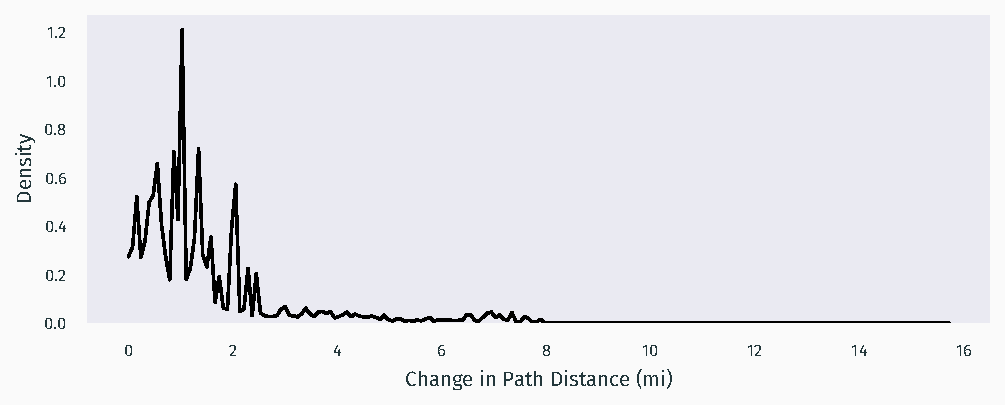
\includegraphics[width=\textwidth]{graphs/path_dists.pdf}
    \end{figure}
\end{frame}

\begin{frame}{Impacted Shortest Paths (3/3)}
    \begin{columns}
        \begin{column}{0.5\textwidth}
            \begin{figure}
                \centering
                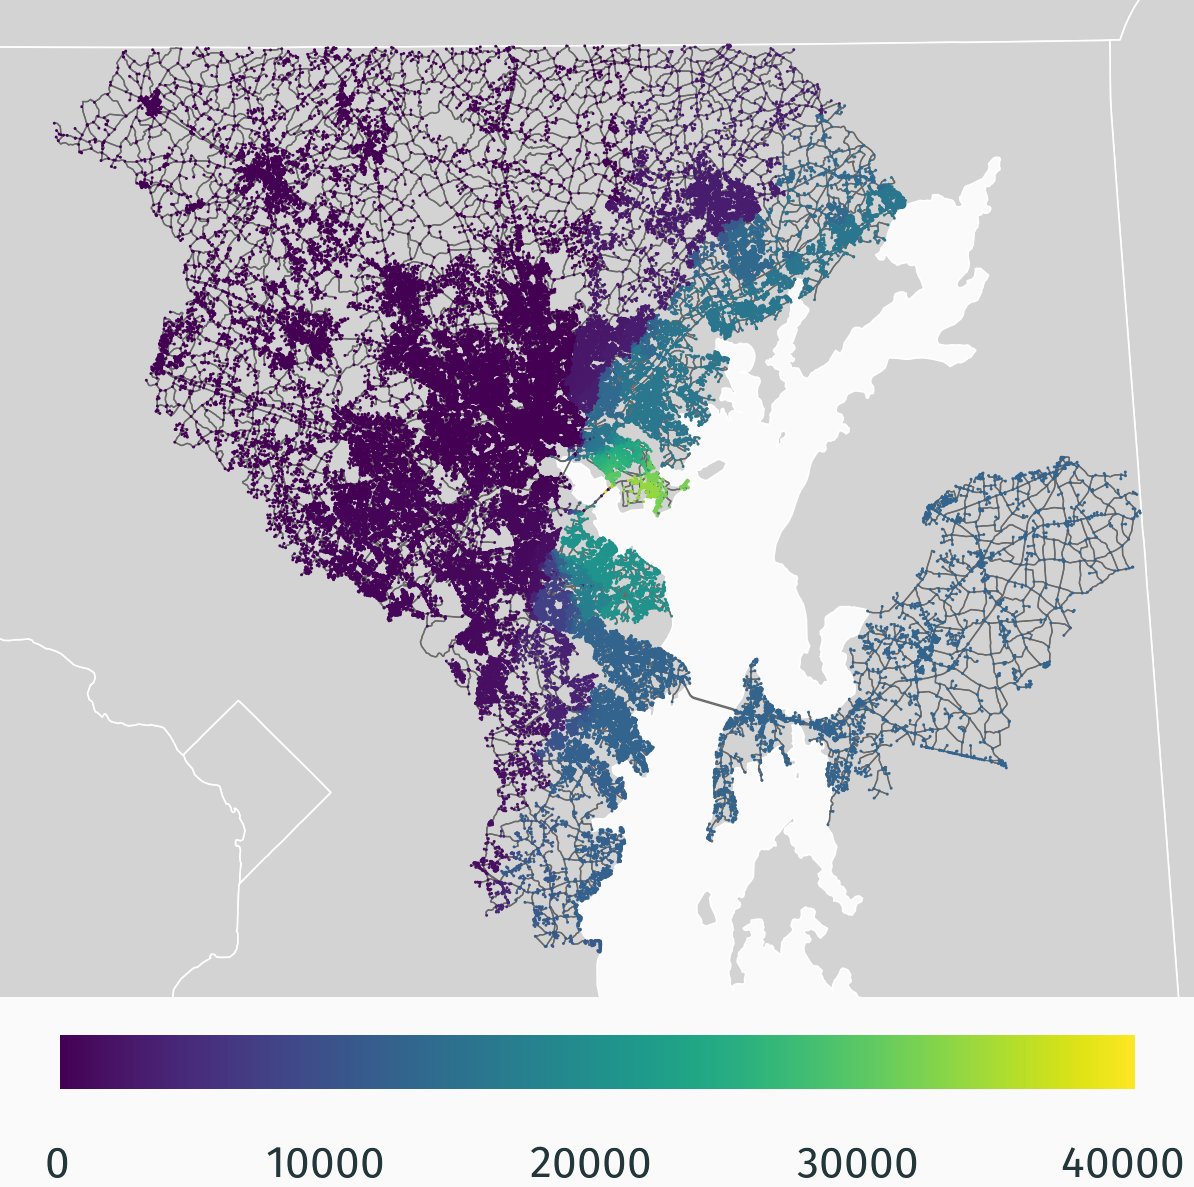
\includegraphics[width=\textwidth]{maps/no_changed_paths.png}
                {\scriptsize Number of Impacted Paths Starting at Node}
            \end{figure}
        \end{column}

        \begin{column}{0.5\textwidth}
            \begin{figure}
                \centering
                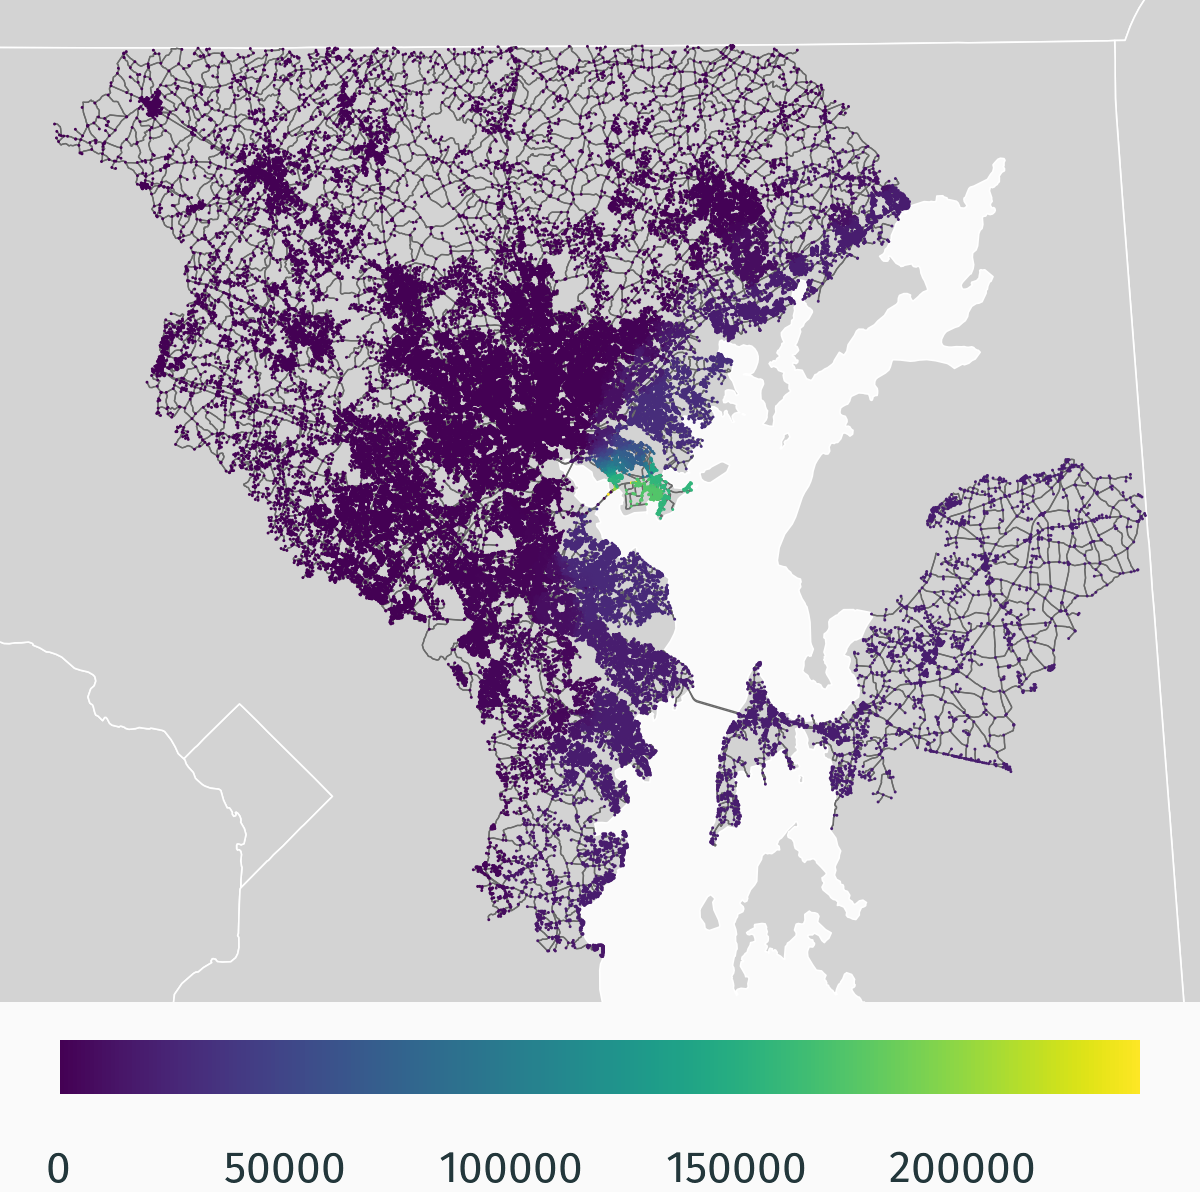
\includegraphics[width=\textwidth]{maps/dist_changed_paths.png}
                {\scriptsize Total Distance Added in Paths Starting at Node}
            \end{figure}
        \end{column}
    \end{columns}
\end{frame}


\section{Conclusion}

\begin{frame}{Conclusions}
    The effects of the bridge collapse were insignificant at a global level, but are significant for individual nodes
    \begin{itemize}
        \item Nodes near the bridge: harder to travel through the network (straightness, closeness, paths from node)
        \item Webs of nodes through the whole network: different levels of traffic importance (eigenvector, betweenness)
    \end{itemize}
\end{frame}

\begin{frame}{Limitations}
    There are many limitations, including
    \begin{itemize}
        \item The network boundary and size is arbitrary
        \item The metrics analyzed are limited and don't include clustering coefficient, largest connected component size, or community devisions, which are standard in attack literature {\tiny \parencite{Xeumei10}}
    \end{itemize}
\end{frame}

\begin{frame}{Further Work}
    Future work could
    \begin{itemize}
        \item Analyze the types of nodes affected 
        \item Look at usage (use average annual daily traffic numbers)
    \end{itemize}
\end{frame}

\begin{frame}[standout]
    Questions?
\end{frame}


\appendix

\begin{frame}[allowframebreaks]{References}
    \printbibliography[heading=none]
\end{frame}

\end{document}
